\section{Gestionare setări}\label{spec:setari}

Aplicația permite setarea de valori predefinite pentru monedă și categorie, care să fie folosite în interpretarea imaginilor. De asemenea, aplicația permite activarea sau dezactivarea colectării de date în mod anonim (Specificația \ref{spec:collecting}). Figura \ref{fig:settingsScreen} prezintă ecranul de modificare a setărilor. 

\begin{figure}[h]
  \centering
  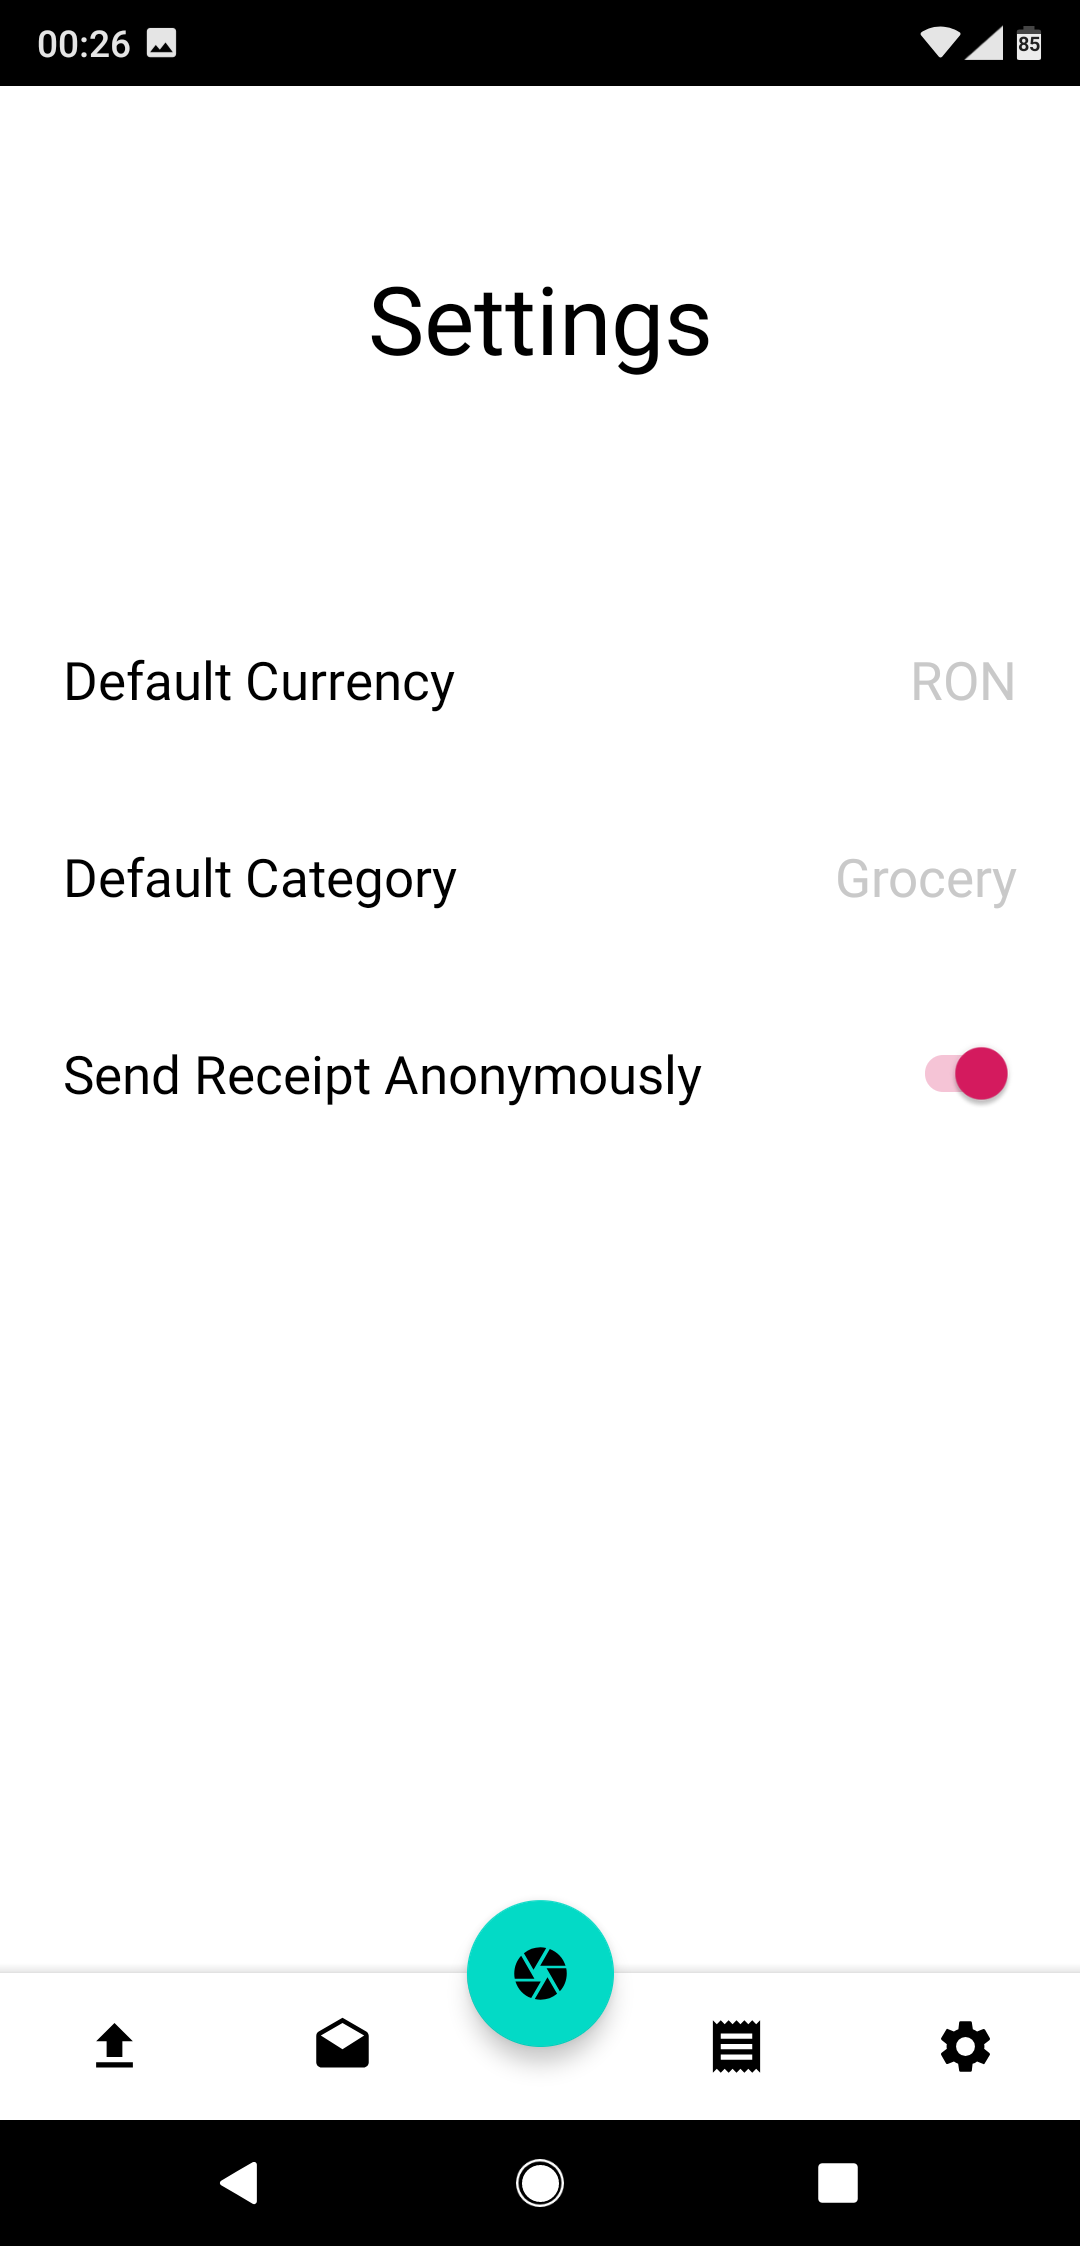
\includegraphics[width=\screenwidth]{SettingsScreen.png}
  \caption{Ecranul de setări}
  \label{fig:settingsScreen}
\end{figure}

\begin{itemize}
\item
  \textbf{Scop}: Modificarea și accesarea unor valori folosite în diferite puncte ale aplicației;
\item
  \textbf{Scenariu de succes}: Modificările făcute de utilizator sunt persistate și pot fi accesate;
\item
  \textbf{Scenarii de eșec}: Modificările nu pot fi persistate; Valorile nu pot fi accesate;
\end{itemize}

\begin{minipage}[t]{0.49\textwidth}

\section*{Mentiuni}
Setările considerate sunt:
\begin{itemize}
  \item
    Valoarea predefinită pentru categorie;
  \item
    Valoarea predefinită pentru monedă;
  \item
    Activarea sau dezactivarea colectării anonime de date;
\end{itemize}    

\end{minipage} \hspace{0.03\textwidth}
\begin{minipage}[t]{0.48\textwidth}
  
\subsection*{Principalul scenariu}
\begin{enumerate}
\item
  Utilizatorul accesează setările
\item
  Utilizatorul modifică valoarea unei setări;
\item
  Noua valoare este persitată și accesibilă;
\end{enumerate}  

\end{minipage}



